%%%%%%%%%%%%%%%%%%%%%%%%%%%%%%%%%%%%%%%%%
% Short Sectioned Assignment LaTeX Template Version 1.0 (5/5/12)
% This template has been downloaded from: http://www.LaTeXTemplates.com
% Original author:  Frits Wenneker (http://www.howtotex.com)
% License: CC BY-NC-SA 3.0 (http://creativecommons.org/licenses/by-nc-sa/3.0/)
%%%%%%%%%%%%%%%%%%%%%%%%%%%%%%%%%%%%%%%%%

%----------------------------------------------------------------------------------------
%	PACKAGES AND OTHER DOCUMENT CONFIGURATIONS
%----------------------------------------------------------------------------------------

\documentclass[paper=a4, fontsize=11pt]{scrartcl} % A4 paper and 11pt font size

% ---- Entrada y salida de texto -----

\usepackage[T1]{fontenc} % Use 8-bit encoding that has 256 glyphs
\usepackage[utf8]{inputenc}
%\usepackage{fourier} % Use the Adobe Utopia font for the document - comment this line to return to the LaTeX default

\usepackage{xcolor}
\usepackage{fancyhdr}
\usepackage{listings, lstautogobble}
\usepackage{comment}

\usepackage{subfigure} % subfiguras

%----------
\lstdefinestyle{customc}{
	belowcaptionskip=1\baselineskip,
	autogobble=true,
	breaklines=true,
	frame=L,
	xleftmargin=\parindent,
	language=C,
	showstringspaces=false,
	basicstyle=\footnotesize\ttfamily,
	keywordstyle=\bfseries\color{green!40!black},
	commentstyle=\itshape\color{purple!40!black},
	mathescape,
	identifierstyle=\color{blue},
	stringstyle=\color{orange},
}

\lstdefinestyle{bashmc}{
	frame=l,
	tabsize=2,
	breaklines=true,
	xleftmargin=\parindent,
	basicstyle=\ttfamily,
	showstringspaces=false,
	commentstyle=\color{red},
	keywordstyle=\color{blue},
	autogobble=true,
}

\lstdefinestyle{r}{
	belowcaptionskip=1\baselineskip,
	autogobble=true,
	breaklines=true,
	frame=L,
	xleftmargin=\parindent,
	language=C,
	showstringspaces=false,
	basicstyle=\footnotesize\ttfamily,
	keywordstyle=\bfseries\color{green!40!black},
	commentstyle=\itshape\color{purple!40!black},
	identifierstyle=\color{blue},
	mathescape,
	stringstyle=\color{orange},
}

\lstdefinestyle{r1}{
	frame=l,
	tabsize=2,
	breaklines=true,
	xleftmargin=\parindent,
	basicstyle=\ttfamily,
	showstringspaces=false,
	commentstyle=\color{red},
	keywordstyle=\color{blue},
	autogobble=true,
}




% ---- Idioma --------

\usepackage[spanish, es-tabla]{babel} % Selecciona el español para palabras introducidas automáticamente, p.ej. "septiembre" en la fecha y especifica que se use la palabra Tabla en vez de Cuadro

% ---- Otros paquetes ----
\usepackage{eurosym} % para el euro
\usepackage{url} % ,href} %para incluir URLs e hipervínculos dentro del texto (aunque hay que instalar href)
\usepackage{amsmath,amsfonts,amsthm} % Math packages
\usepackage{centernot}
%\usepackage{graphics,graphicx, floatrow} %para incluir imágenes y notas en las imágenes
\usepackage{graphics,graphicx, float} %para incluir imágenes y colocarlas

% Para hacer tablas comlejas
%\usepackage{multirow}
%\usepackage{threeparttable}

%\usepackage{sectsty} % Allows customizing section commands
%\allsectionsfont{\centering \normalfont\scshape} % Make all sections centered, the default font and small caps

\usepackage{fancyhdr} % Custom headers and footers
\pagestyle{fancyplain} % Makes all pages in the document conform to the custom headers and footers
\fancyhead{} % No page header - if you want one, create it in the same way as the footers below
\fancyfoot[L]{} % Empty left footer
\fancyfoot[C]{} % Empty center footer
\fancyfoot[R]{\thepage} % Page numbering for right footer
\renewcommand{\headrulewidth}{0pt} % Remove header underlines
\renewcommand{\footrulewidth}{0pt} % Remove footer underlines
\setlength{\headheight}{13.6pt} % Customize the height of the header

\numberwithin{equation}{section} % Number equations within sections (i.e. 1.1, 1.2, 2.1, 2.2 instead of 1, 2, 3, 4)
\numberwithin{figure}{section} % Number figures within sections (i.e. 1.1, 1.2, 2.1, 2.2 instead of 1, 2, 3, 4)
\numberwithin{table}{section} % Number tables within sections (i.e. 1.1, 1.2, 2.1, 2.2 instead of 1, 2, 3, 4)

\setlength\parindent{0pt} % Removes all indentation from paragraphs - comment this line for an assignment with lots of text

\newcommand{\horrule}[1]{\rule{\linewidth}{#1}} % Create horizontal rule command with 1 argument of height





%----------------------------------------------------------------------------------------
%	TÍTULO Y DATOS DEL ALUMNO
%----------------------------------------------------------------------------------------

\title{	
\normalfont \normalsize 
\textsc{\textbf{Metaheurísticas (2016-2017)} \\ Grado en Ingeniería Informática \\ Universidad de Granada} \\ [25pt] % Your university, school and/or department name(s)
\horrule{0.5pt} \\[0.4cm] % Thin top horizontal rule
\huge Practica 2: APC \\ % The assignment title
\horrule{2pt} \\[0.5cm] % Thick bottom horizontal rule
}

\author{Samuel Cardenete Rodríguez.  \\Correo: samuelcr1995@correo.ugr.es \\ DNI: 75934968P} % Nombre y apellidos

\date{\normalsize\today} % Incluye la fecha actual

%----------------------------------------------------------------------------------------
% DOCUMENTO
%----------------------------------------------------------------------------------------

\begin{document}

\maketitle % Muestra el Título

\newpage %inserta un salto de página

\tableofcontents % para generar el índice de contenidos

\listoffigures



\newpage





\section{Formulación del problema. APC}

\subsection{Introducción}
El problema a abordar en esta práctica consiste en el aprendizaje de pesos por características (APC). \\ 
Se trata de un problema de búsqueda con codificación real en el espacio n-dimensional, siendo n el número de características.\\ 

Estamos delante de un problema de Machine Learning, mediante el cuál dado un conjunto de datos no etiquetados obtengamos una etiqueta para cada uno de los datos (por ejemplo, determinar a partir de determinados parámetros si se tiene o no cáncer) bajo una tasa de acierto (función objetivo), siempre a maximizar.\\ 

\subsection{Objetivos}
Como objetivo principal del problema, ajustaremos un conjunto de ponderaciones o pesos asociados al conjunto total de características, utilizando para ello un conjunto de datos de entrenamiento (ya etiquetados), de tal forma que los clasificadores que se construyan a partir de él sean mejores.\\ 

APC asigna valores reales a las características, de tal forma que se describe o pondera la relevancia de cada una de ellas al problema del aprendizaje.

Para la resolución del problema, nos basaremos en optimizar el rendimiento de un clasificador basado en vecinos cercanos a partir de la inclusión de pesos asociados a las características del problema que modifican su valor en el momento de calcular las distancias entre ejemplos. En nuestro caso, el clasificador considerado será el 1-NN (vecino más cercano). Para ello adaptaremos las dos siguientes técnicas metaheurísticas:

\begin{itemize}
	\item Enfriamiento Simulado: Implementación del Enfriamiento llevando a cabo un esquema de enfriamiento de Cauchy modificado. Para la generación de vecinos se emplea el el movimiento de cambio por mutación normal.
	
	\item Búsqueda local reiterada: Implementamos la ILS generando la solución inicial de forma aleatoria y aplicamos búsquedas locales reiteradas, aplicando mutaciones sobre la mejor solución obtenida.
	
	\item Evolución diferencial: Implementamos el algoritmo basado en modelo evolutivo. Generaremos dos algoritmos, uno con formula de mutación \textit{DE/Rand/1} y otro \textit{DE/current-to-best/1}, ambos emplearan recombinación binomial.
\end{itemize}


Tras esto realizaremos un estudio comparativo de los resultados obtenidos por las distintas técnicas metaheurísticas.

\section{Función objetivo}
Debido a la falta de diversidad en los datos a evaluar, realizaremos modificaciones en el método de evaluación de los datos.\\ 

Ahora consideraremos un nuevo criterio basado en la simplicidad del clasificador diseñado basado en la minimización del número de características a utilizar en el clasificador final.

De tal forma que ahora nuestra función objetivo consistirá en la agregación del porcentaje de clasificación realizado por la solución y el porcentaje de características (pesos) inferiores a 0.1 obtenidas.

Además, se establece una ponderación entre estos dos agregados, de forma que los dos tengan igual importancia, es decir, $\alpha=0.5$.\\ 
La función objetivo quedaría así:
\[
tasa \ clasificacion = 100*\frac{\text{nº instancias bien clasificadas}}{\text{nº instancias totales}}
\]

\[
tasa\ reduccion = 100*\frac{\text{nº valores}\ w_i > 0.1}{\text{nº valores totales}}
\]

\[
funcion \ evaluacion = tasa\ clasificacion*\alpha + (1-\alpha)*tasa\ reduccion
\]

En nuestro caso, como deseamos darle igual importancia dando a la reducción como a la clasificación, indicaremos un $\alpha=0.5$.\\ 

Puesto que ahora deseamos que sólo se tengan en cuenta aquellos pesos cuyo valor sea superior o igual a 0.1, será necesario modificar la función 'CalcularDistancia' que emplea 1-nn para que aquellos pesos cuyo valor sea inferior a 0.1 sean ignorados; por lo que el pseudocódigo sería el siguiente:

\begin{lstlisting}[ style=r]
//Calcular la distancia entre dos cromosomas
// teniendo en cuenta el vector de pesos:
Calcular distancia cromosoma A y B:
	Para cada i $\in$ Atributos(A) y j $\in$ Atributos(B)
		Si $Pesos_i >= 0.1$
			distancia = distancia + $\sqrt{Pesos_i*(i-j)^2}$
	Fin para cada
	
	Devolver distancia
\end{lstlisting}


\section{Mecanismo de validación}
El mecanismo empleado para la validación de las soluciones obtenidas por los algoritmos es la validación cruzada.\\ 

Consiste en la realización de validación cruzada donde realizamos 5 particiones de los datos, de forma que cada partición es del mismo tamaño que el conjunto originar de datos.\\ 
Ahora, para realizar la validación, para cada partición, emplearemos $4/5$ de los datos para train, es decir, para obtener el modelo de aprendizaje; y el conjunto restante ($1/5$) para evaluar el modelo obtenido.\\ 

De esta forma el esquema de evaluación en cada una de las 5 iteraciones de la validación cruzada será el siguiente:



\begin{figure}[H]
	\centering
	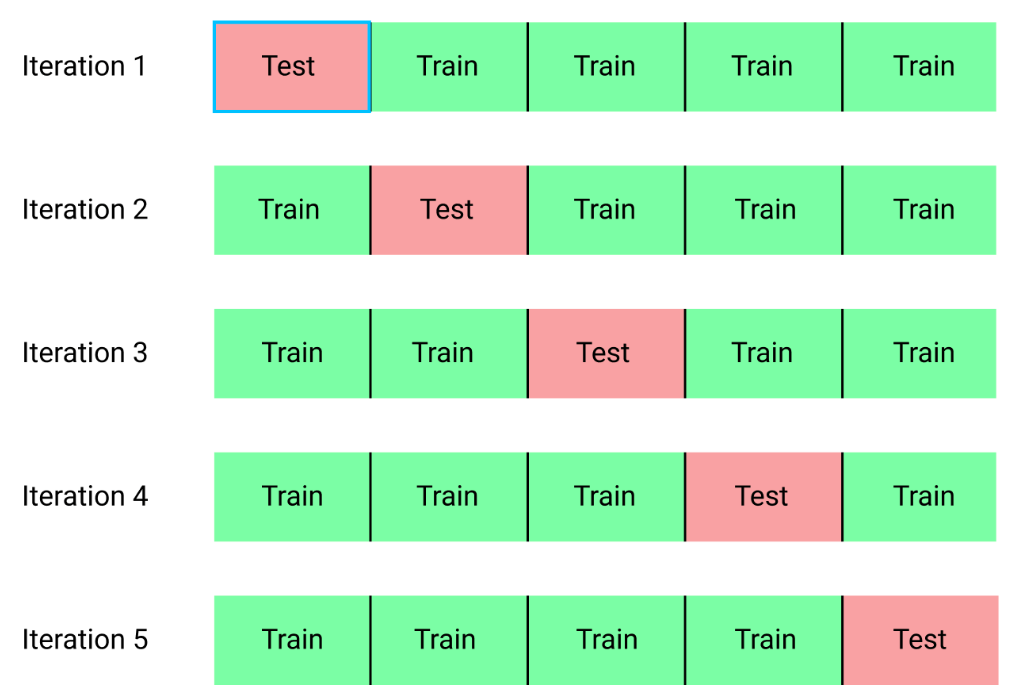
\includegraphics[scale=0.35]{CV.png}  
	\caption{5fold CrossValidation} \label{5fold CrossValidation}
\end{figure}

De esta forma, siguiendo dicho esquema de validación, el pseudo código del particionamiento sería el siguiente:

\begin{lstlisting}[ style=r]
Particionamiento de datos $Datos$
	//Mezclamos el conjunto de datos para mejorar la variabilidad:
	sample(datos)
	//Dividimos en cinco trozos los datos
	tamFold = Datos/5
	
	Desde i=0 hasta cinco
		
		$Test_i = Datos[i*tamFold, i*tamFold+tamFold]$
		$Train_i = Datos - Test_i$
		
		particiones $\leftarrow (Train_i, Test_i)$
	Fin Deste
	
	Devolver Particiones	
fin para cada
\end{lstlisting}


\section{Algoritmos empleados al problema.}

\subsection{Algoritmos comunes}
Representación y explicación de los principales algoritmos comunes (mutación...) así como su estructura en pseudocódigo.

\subsection{Generador de soluciones aleatorias}
En el ámbito de nuestro problema APC, la representación de una solución corresponde a un vector de pesos W.
Para determinados algoritmos como los genéticos o la búsqueda local partimos de una solución aleatoria, es decir, un vector de pesos con componentes aleatorias generadas entre un intervalo $[0,1]$ (de esta forma ahorramos la normalización). El pseudocódigo sería el siguiente:

\begin{lstlisting}[ style=r]

Desde i hasta numero atributos
	SolucionInicialGenerarAleatorio $\Leftarrow$ Aleatorio (0,1)
Fin Desde

Devuelve SolucionInicial
\end{lstlisting}

De esta forma obtenemos un cromosoma aleatorio ya normalizado.

\subsection{Normalización de datos.}
Dados unos conjuntos de datos a utilizar como base de pruebas para nuestro problema (wdbc, sonar...), para no priorizar unos datos sobre otros es necesario la normalización de los datos en un intervalo $[0,1]$. Para ello, empleo un script en R, de forma que leemos los ficheros .arff, y utilizamos la función normalizarDatos para guardarlos en un .csv ya normalizados, de forma que dado un valor $x_j$ perteneciente a un atributo j del ejemplo $x$, y sabiendo que el dominio del atributo j es $[Min_j, Max_j]$, el valor normalizado de $x_j$ es:
\[
x_j^N = \frac{x_j -Min_j}{Max_j - Min_j}
\]



\subsection{Función de evaluación}
Implementación de la función de evaluación 1-NN explicada en la descripción anteriormente.\\ 
El pseudocódigo es el siguiente:

\begin{lstlisting}[ style=r]
1-NN(train, test, pesos)

//Recorremos el conjunto test:
Para todo $a_i \in$ Test
	//inicializamos las distancias minimas al enemigo
	// y al amigo a infinito
	$d_{min} = \infty$

	
	//Ahora recorremos el conjunto train
	// calculando las distancias, buscando el min
	
	Para todo $b_i \in$ Train
		Si $a_i \neq b_i$ //leave one out
			Si (calculaDistancia($a_i$, $b_i$) < $d^{enemigo}_{min}$)
				$d_{min} =$ calculaDistancia($a_i$, $b_i$, pesos)
			
			Fin Si
	Fin para todo
	
	
	
	

Fin para todo

tasa = 100*etiquetas bien clasificadas / numero total de etiquetas
//Ahora calculamos la tasa de clasificacion,
// la tasa de reduccion y la func. objetivo:
$tasa\ reduccion = 100*\frac{\text{nº valores}\ w_i > 0.1}{\text{nº valores totales}}$
$funcion \ evaluacion = tasa\ clasificacion*\alpha + (1-\alpha)*tasa\ reduccion$

Devolver func. evaluacion
\end{lstlisting}


\subsection{Generación de vecinos}
En el esquema de generación de vecinos, necesario para la Búsqueda local, la Búsqueda local iterativa y el enfriamiento simulado, emplea un movimiento de cambio por mutación Normal, Mov(W,$\sigma$), deforma que a una característica del atributo se le suma un valor aleatorio obtenido a partir de una distribución normal de media 0 y desviación típica 0.3.\\ 

El pseudocódigo del algoritmo quedaría tal que así:

\begin{lstlisting}[ style=r]
Generar vecino (Pesos, $a_i$ = atributo a modificar)
	//Obtenemos un valor de la distribucion normal mencionada:
	aleatorio = Distribucion normal($media = 0$, $\sigma = 0.3$)
	//modificamos el atributo $a_i$ de los pesos:
	Pesos($a_i$) = Pesos($a_i$) + aleatorio
	
	//truncamos si es necesario para tener los valores normalizados 
	//entre $[0,1]$:
	
	Si Pesos($a_i$) < 0
		Pesos($a_i$) = 0
	Si Pesos($a_i$) > 1
		Pesos($a_i$) = 1
		
	Devolvemos Pesos
\end{lstlisting}
De esta forma tendremos un vecino generado.

\subsection{Operador cruce BLX}
Para el algoritmo genético BLX es necesario la implementación de dicho cruce BLX-$\alpha$, donde en nuestro caso $\alpha = 0.3$.
Dados dos cromosomas $p_1,  p_2$ pertenecientes a los padres, generamos dos descendientes $h_1, h_2$
de la siguiente forma descrita en pseudocódigo:

\begin{lstlisting}[ style=r]
CruceBLX entre $p_1$ y $p_2$
	//Obtenemos los atributos maximos y minimos para cada padre:
	$a_{max}^1 , a_{min}^1 \in p_1$
	$a_{max}^2, a_{min}^2 \in p_2$
	
	//Ahora obtenemos el maximo y el minimo de los dos padres:
	Max($a_{max}^1, a_{max}^2$)
	Min($a_{min}^1, a_{min}^2$)
	
	//Ahora generamos el intervalo I del cual generaremos aleatoriamente a los dos hijos:
	I = [Min($a_{min}^1, a_{min}^2$)-(Max($a_{max}^1, a_{max}^2$-Min($a_{min}^1, a_{min}^2$)*0.3,Max($a_{max}^1, a_{max}^2$)+(Max($a_{max}^1, a_{max}^2$-Min($a_{min}^1, a_{min}^2$)*0.3 ]
	
	//Creamos a los dos hijos $h_1,  h_2$
	Para cada atributo $a_1^i \in h_1$ y $a_2^i \in h_2$
		$a_1^i$ = Aleatorio (I)
		$a_2^i$ = Aleatorio (I)
	fin para cada
	
	devolvemos $a_1$ y $a_2$
		
\end{lstlisting}

De esta forma para cada pareja de padres, obtenemos una pareja de hijos.


\subsection{Torneo Binario}
La función torneo binario realiza un torneo entre dos padres (cromosomas) aleatorios, es decir, de entre esos dos padres, elige aquel que posea una mayor tasa de clasificación, o lo que es lo mismo, el mejor de los dos.\\ 
Genera tantos padres por torneo binario como se le indique. El pseudocódigo sería el siguiente, recibiendo una población y sus tasas correspondientes:

\begin{lstlisting}[ style=r]

TorneoBinario Poblacion, Tasas
	Desde i hasta $N_{padres a generar}$
		//Obtenemos dos padres de forma aleatoria:
		p1 = aleatorio(Poblacion)
		p2 = aleatorio(Poblacion) distinto de p1
		
		//Ahora nos quedamos con el que tenga mejor tasa de los dos:
		mejores padres $\Leftarrow$ Max(Tasas(p1), Tasas(p2))
	Fin desde
	
	Devolver mejores padres

\end{lstlisting}

De esta forma obtenemos al final un número de padres deseados obtenidos mediante torneo binario, que emplearemos para un posterior cruce en los algoritmos genéticos y meméticos correspondientes.


\subsection{Cálculo temperatura inicial}
Para la generación del esquema de enfriamiento, una de las principales características es la temperatura inicial sobre la cuál comienza a enfriar el algoritmo.

La temperatura inicial la establecemos como la relación entre un porcentaje ($\mu$) del coste de una solución inicial aleatoria y el negado del logaritmo neperiano de la probabilidad de aceptar una solución un $\mu$ por 1 peor que la inicial.

El pseudocódigo sería el siguiente:
\begin{lstlisting}[ style=r]

CalculoTemperaturaInicial $\mu$, Solucion inicial, $\phi, datos$
	//calculamos el coste:
	$C_{\text{solucion inicial}}$ = knn(datos, Solucion inicial)
	
	$T_{inicial} = \frac{\mu*C_{\text{solucion inicial}}}{-ln(\phi)}$

	Devolver $T_{inicial}$

\end{lstlisting}

\subsection{Mutación para ILS}
Para la ILS emplearé el mismo cambio por mutación descrito anteriormente, pero esta vez realizamos el cambio sobre 'T' genes de la solución a mutar; por tanto, el pseudocódigo será el siguiente:


\begin{lstlisting}[ style=r]
Mutacion ILS (Pesos, atributos a modificar)
	Para cada a_i en 'atributos a modificar'
		//Obtenemos un valor de la distribucion normal mencionada:
		aleatorio = Distribucion normal($media = 0$, $\sigma = 0.3$)
		//modificamos el atributo $a_i$ de los pesos:
		Pesos($a_i$) = Pesos($a_i$) + aleatorio
		
		//truncamos si es necesario para tener los valores normalizados 
		//entre $[0,1]$:
		
		Si Pesos($a_i$) < 0
			Pesos($a_i$) = 0
		Si Pesos($a_i$) > 1
			Pesos($a_i$) = 1
	Fin Para Cada
		
	Devolvemos Pesos
\end{lstlisting}




\section{Estructuras de los principales métodos de búsqueda}

\subsection{Búsqueda Local}
La implementación de la búsqueda local consiste en emplear una técnica de búsqueda mediante explotación aplicada a nuestro problema, de forma que nos permita explotar una solución localmente, permitiendo así maximizar la tasa evaluación de una solución de forma local.\\ 

Como \textbf{criterio de parada} cuando se ejecute como algoritmo individual, se detendrá tras haber generado 20* (numero veces el número de características) vecinos, o cuando se hayan realizado 15000 evaluaciones (llamadas al 1-NN).

Además, como modificación, parametrizamos el número máximo de evaluaciones, de forma que cuando ejecutemos ILS le indiquemos un máximo de 1000 evaluaciones en cada llamada a BL

El pseudocódigo sería el siguiente:

\begin{lstlisting}[ style=r]

Busqueda Local (Conjunto de datos: Data)
	//Primero generamos una solucion inicial de forma aleatoria
	$S_{inicial} = GenerarSolucionAleatoria()$
	//Y calculamos la tasa
	$T_{inicial} =$ knn(Data, Data, $S_{inicial}$)
	
	
	//Inicializamos la primera como mejor solucion actual:
	$S_{mejor} = S_{inicial}$
	//Y guardamos la mejor tasa como esta:
	$T_{mejor} = T_{inicial}$
	
	//Llevamos cuenta del numero de evaluaciones que llevamos:
	numero evaluaciones = 1
	
	
	//Empezamos a generar vecindario con la solucion actual 
	// hasta que se cumplan los criterios de parada:

	Mientras (numero evaluaciones < MAX EVALUACIONES) y (vecinos generados < 20*(Numero genes cromosoma)
	
		//vamos generando el vecindario:
		Si hay_que_generar_nuevo_vecindario
			//rellenamos una cola de indices aleatorios desde con los genes a mutar
			vecinos por generar = Shuffle(Indices de genes)
			hay_que_generar_nuevo_vecindario = false
		Sino
			//Generamos un vecino correspondiente sacando
			// un elemento de la cola anterior para
			//Indicar que gen mutar:
			nuevo vecino = generarVecino($S_{mejor}$, vecinos por generar)
			vecinos generados +1
			
			Si (Tasa(nuevo vecino) > $T_{mejor}$)
				$S_{mejor}$ = nuevo vecino
				$T_{mejor}$ = knn(Data, Data, nuevo vecino)
				
				numero evaluaciones+1
				
				//Indicamos que genere un nuevo vecindario
				hay_que_generar_nuevo_vecindario = true
			Fin Si
			
		Fin Sino
		
		//Hemos recorrido un vecindario sin mejora
		Si estaVacia(vecinos por generar)
			hay_que_generar_nuevo_vecindario = true
		Fin Si
		
	Fin Mientras
	
	Devolver $S_{mejor}$
\end{lstlisting}


\subsection{Enfriamiento Simulado}
El algoritmo de enfriamiento simulado empleará como temperatura inicial el procedimiento descrito en el apartado anterior, además, seguirá el siguiente esquema de enfriamiento:
\subsubsection{Esquema de enfriamiento}
Para la realización del algoritmo empleamos un esquema de enfriamiento de Cauchy modificado, es decir, una modificación de las dos ecuaciones diferenciales de Cauchy. El esquema tradicional consiste en que sea k el enfriamiento actual, tenemos que:
\[
T_k = \frac{T_0}{k+1}
\]

En nuestro caso, incluiremos un parámetro $\beta$ asociado a la temperatura actual, de forma que la temperatura en una iteración posterior sea:
\[
T_k + 1=\frac{T_k}{1+\beta*T_k} 
\]

Donde el parámetro $\beta$ es la relación entre la diferencia de las cotas de temperatura entre el producto de esas cotas y el nº de enfriamientos a realizar:
\[
\beta = \frac{T_0-T_f}{M*T_0*T_k}
\]

\subsubsection{Algoritmo ES}
Una vez descritos tanto la generación de la temperatura inicial, así como del esquema de enfriamiento a realizar, es pseudocódigo del algoritmo será el siguiente:

\begin{lstlisting}[ style=r]

EnfriamientoSimulado (Datos)
	//En primer lugar generamos una solucion de forma
	//aleatoria (pesos intervalo [0,1]):
	$S_{inicial}$ = generaSolucionAleatoria()
	$S_{actual} = S_{inicial}$
	$S_{mejor} = S_{actual}$
	
	//Ahora calculamos la temperatura inicial y la final:
	$T_0$ = $T_k$ = CalculoTemperaturaInicial($\mu$=0.3, $S_{inicial}$, $\phi$=0.3, Datos)
	$T_f$ = 0.001
	//Definimos el num. max. de vecinos a generar:
	maximos vecinos = $10*n\ | n=\text{tamaño del problema}$
	//Definimos el num. max. de enfriamientos (M):
	$M$ = $\frac{15000}{maximos vecinos}$
	
	//Comenzamos a realizar los enfriamientos, hasta alcanzar el max.
	// de endriamientos o hasta que no se produzcan mas exitos:
	Mientras (enfriamientos < M) y (exitos \ne 0)
		vecinos = exitos = 0
		
		Mientras (vecinos < maximos vecinos) y (exitos < maximos exitos)
			vecino = generarVecino(solucion Actual)
			
			Si ($C(vecino)- C(S_{actual}) >0$) o $(U(0,1) \le e^{\frac{-(C(vecino)-C(S_{actual})}{\text{enfriamientos}*T_k}}) $
				
				$S_{actual}$ = vecino
				exitos \leftarrow exitos +1
				
				Si ($C(S_{actual})$ > $C(S_{mejor})$)
					$S_{mejor} = S_{actual}$
				Fin Si
			Fin Si
		Fin Mientras
		//Enfriamos:
		$\beta = \frac{T_0-T_f}{M*T_0*T_k}$
		$T_k + 1=\frac{T_k}{1+\beta*T_k} $
		enfriamientos $\leftarrow$ enfriamientos+1
		
	Fin Mientras
	
	Devolver $S_{mejor}$

\end{lstlisting}



\subsection{Búsqueda local reiterada}
La realización del algoritmo de búsqueda reiterada se basa en generar una solución aleatoria y aplicar Búsquedas locales reiteradas, de forma que obtengamos una solución optimizada.\\ 
Una vez obtenida dicha solución estudiamos si es mejor que la encontrada hasta el momento y realizamos una mutación siguiendo el esquema $Mov(W,\sigma)$ sobre la mejor de las dos, de forma que volvamos a aplicar la búsqueda local sobre dicha solución.\\ 

Respecto al proceso de mutación, realizaremos un cambio brusco, de forma que aplicamos la mutación sobre un conjunto de $t$ características escogidas aleatoriamente en la solución.\\ 
Para la llamada a la búsqueda local, le indicaremos que realice un máximo de 1000 iteraciones por búsqueda local, de esta forma, el máximo de iteraciones a realizar por nuestro algoritmo ILS serán 15, de forma que si en cada iteración realizamos una búsqueda local con 1000 llamadas a la función 0bjetivo, en total realizaremos 15000 llamadas a la función objetivo.

\subsubsection{algoritmo ILS}
Siguiendo el proceso y esquema de mutación descrito anteriormente el pseudocódigo será el siguiente:

\begin{lstlisting}[ style=r]

ILS (Datos)
	//En primer lugar generamos una solucion de forma
	//aleatoria (pesos intervalo [0,1]):
	$S_{inicial}$ = generaSolucionAleatoria()
	$S_{actual} = BL(S_{inicial})$
	$S_{a_mutar} = S_{actual}$
	$S_{mejor} = S_{actual}$
	
	//Al haber hecho una BL adelantada, iteramos hasta 14:
	Desde i=1 hasta 14
		//mutamos un conjunto de t atributos aleatorios
		$S_{mutada}$ = mutacionILS($S_{a_mutar}$)
		
		//Aplicamos BL:
		$S_{actual}$ = BL($S_{mutada}$)
		
		//Si la solucion mejora, actualizamos:
		If(C($S_{mutada}$) > C($S_{actual}$))
			$S_{actual} = S_{mutada}$
			$S_{a_mutar} = S_{actual}$
		Fin If
	Fin Desde
	
	Devolver \text{Mejor solucion encontrada}	
\end{lstlisting}

\subsection{Evolución diferencial}
Se trata de un modelo evolutivo para optimización con parámetros reales que enfatiza en la mutación y en el operador de cruce a posteriori.\\ 
Para al obtención del vector de mutación emplearemos dos modelos de generación:

\begin{itemize}
	\item \textbf{DE/Rand/1}: Para la mutación, en este caso obtenemos tres padres (tres individuos de la generación actual) escogidos aleatoriamente, de forma que siendo r1, r2 y r3 dichos individuos, G el índice de la generación actual y F un factor (porcentaje) que multiplica la diferencia entre dos padres:
	calculamos dicho vector de la siguiente forma:
	\[
	V_{i,g}=X_{r1, G}+F*(X_{r2,G}-X_{r3,G})
	\]
	
	\item \textbf{DE/current-to-best}: Para calcular el vector de mutación esta vez obtenemos dos padres (aleatoriamente también), pero además ahora incrementamos el gen teniendo en cuenta la mejor solución, de forma que lo calculamos así:
	\[
	V_{i,g}=X_{i, G}+F*(X_{mejor,G}-X_{i,G})+ F*(X_{r1,G}-X_{r2,G})
	\]
\end{itemize}

Cuando terminamos de actualizar el vector de mutaciones, comprobamos que los genes se encuentran normalizados en el intervalo [0,1], de no ser así, los normalizamos.\\ 

El pseudocódigo resultante de la evolución diferencial para DE/Rand/1 sería el siguiente:
\begin{lstlisting}[ style=r]

Evolucion diferencial Rand (Datos)
	//En primer lugar generamos una poblacion de 50 individuos
	// de forma aleatoria
	Desde i = 0 hasta i < 50
		Poblacion actual <- generaSolucionAleatoria()
	Fin Desde
	
	//Ahora realizamos una evaluacion de la poblacion:
	Para cada $P_i \in $ poblacion actual
		tasas actuales $\Leftarrow$ knn(Datos, $P_i$)
	Fin para cada
	
	//Como condicion de parada tendremos 15000 evaluaciones:
	Mientras (num. evaluaciones < 15000)
		//Recorremos la poblacion actual:
		Desde i=1 hasta 50
			//Elegimos tres individuos de forma aleatoria de la
			//poblacion actual:
			r1 = aleatorio(poblacion actual)
			r2 = aleatorio(poblacion actual) $|\ r2 \ne r1$
			r3 = aleatorio(poblacion actual) $\ r3 \ne r2 \wedge r3 \ne r1$
			
			//Recorremos los genes del individuo $I_i$
			Para cada Gen $Xj$ en $I_i$
				//mutamos teniendo segun DE/Rand/1
				Si(aleatorio <= PROB.CRUCE=0.5 || aleatorio == i)
					mutado $\leftarrow$ $X_{r1,j}+F*(X_{r2,j}-X_{r3,j})$
				sino
					mutado $\leftarrow X_j$
			Fin para cada
			
			//Lo evaluamos:
			coste_mutacion = knn(mutacion)
			
			//normalizamos por si nos hemos salido del intervalo:
			Normalizar(mutado)
			
			Si coste_mutacion > tasas actuales($I_i$)
				//Lo aniadimos a una nueva poblacion:
				nueva poblacion $\leftarrow$ mutado
				tasas nueva poblacion $\leftarrow$ coste_mutacion
			Sino
				nueva poblacion $\leftarrow$ $I_i$
				tasas nueva poblacion $\leftarrow$ tasas(I_{i})
			Fin Si
		Fin Desde
		
		//Actualizamos la poblacion:
		poblacion actual = nueva poblacion
		
	Fin Mientras
	
	
	
	Devolver \text{Mejor solucion encontrada}	
\end{lstlisting}

Como podemos observar, el tamaño empleado para la población es de 50 individuos.\\ 
El pseudo código de la evolución diferencial siguiendo una mutación 'DE/current-to-best' sería el siguiente:

\begin{lstlisting}[ style=r]

Evolucion diferencial DE/current-to-best (Datos)
	//En primer lugar generamos una poblacion de 50 individuos
	// de forma aleatoria
	Desde i = 0 hasta i < 50
		Poblacion actual <- generaSolucionAleatoria()
	Fin Desde
	
	//Ahora realizamos una evaluacion de la poblacion:
	Para cada $P_i \in $ poblacion actual
		tasas actuales $\Leftarrow$ knn(Datos, $P_i$)
	Fin para cada
	
	//Como condicion de parada tendremos 15000 evaluaciones:
	Mientras (num. evaluaciones < 15000)
		//Recorremos la poblacion actual:
		Desde i=1 hasta 50
			//Elegimos dos individuos de forma aleatoria de la
			//poblacion actual:
			r1 = aleatorio(poblacion actual)
			r2 = aleatorio(poblacion actual) $|\ r2 \ne r1$

			
			//Recorremos los genes del individuo $I_i$
			Para cada Gen $Xj$ en $I_i$
				//mutamos teniendo segun DE/current-to-best
				Si(aleatorio <= PROB.CRUCE=0.5 || aleatorio == i)
					mutado $\leftarrow$ $X_{j}+F*(X_{mejor,j}-X_{j})+F*(X_{r1,j}-X_{r2,j})$
				sino
					mutado $\leftarrow X_j$
				
				
			Fin para cada
			
			//Lo evaluamos:
			coste_mutacion = knn(mutacion)
			
			//normalizamos por si nos hemos salido del intervalo:
			Normalizar(mutado)
			
			Si coste_mutacion > tasas actuales($I_i$)
				//Lo aniadimos a una nueva poblacion:
				nueva poblacion $\leftarrow$ mutado
				tasas nueva poblacion $\leftarrow$ coste_mutacion
			Sino
				nueva poblacion $\leftarrow$ $I_i$
				tasas nueva poblacion $\leftarrow$ tasas(I_{i})
			Fin Si
		Fin Desde
		
		//Actualizamos la poblacion:
		poblacion actual = nueva poblacion
		
	Fin Mientras

	Devolver \text{Mejor solucion encontrada}	
\end{lstlisting}




\subsection{AGG BLX}
El AGG BLX se trata de un algoritmo que implementa un esquema de evolución generacional elitista, mediante un esquema de reemplazamiento generacional, es decir, la nueva generación reemplaza en cada iteración completamente a la generación actual.\\ 
Como operador de selección se implementará el torneo binario ya descrito anteriormente, para la elección de los mejores padres a cruzar.\\ 

El operador de cruce es el BLX, descrito anteriormente, para generar en cada cruce a partir de dos padres dos descendientes. La probabilidad de cruce será de 0.7.\\ 

Para la mutación, se empleará la función generarVecino descrita anteriormente, bajo una probabilidad de mutación en población de un 0.001.\\ 

Por último el criterio de parada del algoritmo es no superar las 15000 evaluaciones de la función objetivo (1-NN).




\subsection{AM-(10, 0.1mej)}
Consiste en que dado el algoritmo AGG-CA mencionado, cada 10 generaciones aplicamos una búsqueda local sobre los 0.1*N mejores cromosomas de la población.\\ 
El pseudocódigo sería el siguiente:


\begin{lstlisting}[ style=r]

AM-(10, 0.1mej) (Data)
//Creamos una poblacion de 10 individuos aleatoria:
Desde i = 0 hasta i < 10
	Poblacion actual <- generaSolucionAleatoria()
Fin Desde

Para cada $P_i \in $ poblacion actual
	tasas actuales $\Leftarrow$ knn(Data, Data, $P_i$)
Fin para cada

//empezamos generacion tras generacion hasta cumplir
//El criterio de parada:
Mientras (num. evaluaciones < 15000)
	//Calculamos el mejor padre de la poblacion actual:
	$Padre_{mejor}$ = Max(tasas poblacion actual)
	
	//Obtenemos los padres (parejas) a cruzar, 
	//con una probabilidad de cruce del 70%
	parejas a cruzar = 0.7 * 10
	
	//Llamamos al torneo binario, obteniendo los padres deseados, 
	// en este caso, el doble del tamanio de la poblacion actual, puesto que 
	// el operador de cruce CA devuelve un unico descendiente.
	padres a cruzar = torneoBinario(poblacion actual)
	//Realizamos los cruces, obteniendo dos hijos por cruce
	Desde i = 0 hasta i < parejas a cruzar
		nueva poblacion $\Leftarrow$ cruceAritmetico($pareja_i, pareja_{i+1}$)
	Fin Desde
	
	//Aniadimos los padres que no se han cruzado hasta llegar 
	// a una nueva poblacion de 10:
	Mientras Tam(nueva poblacion) < 10
		nueva poblacion $\Leftarrow$ padres no se han cruzado
	Fin Mientras
	
	//Calculamos el numero de individuos a mutar, con
	// una probabilidad de 0.001:
	individuos a mutar = 0.001 * 10
	
	//Mutamos de forma aleatoria los n individuos a mutar:
	Desde i = 0 hasta i < individuos a mutar
		nueva $poblacion_{aleatorio}$ = generarVecino (nueva $poblacion_{aleatorio}$)
	Fin Desde
	
	//Calculamos las tasas de la nueva poblacion
	Para cada $P_i \in $ nueva poblacion
		nuevas tasas $\Leftarrow$ knn(Data, Data, $P_i$)
	Fin para cada
	
	//Si hemos perdido al mejor padre lo cambiamos por 
	//el peor de la poblacion.
	Si (hemos perdido al mejor padre)
		Min(tasas actual) = mejor padre
	Fin Si
	
	//La nueva poblacion es ahora la actual:
	poblacion actual = nueva poblacion
	tasas actual = nuevas tasas
	
	
	//Si ya llevamos 10 generaciones aplicamos la busqueda local:
	Si (generaciones es multiplo de 10)
		Para cada $c_i$ \in 0.1*poblacion actual
			$c_i$ = BL (Data, $c_1$)
			Tasas actual ($c_i$) = Tasa($c_i$)
		Fin para cada
	Fin Si


Fin Mientras


Devolver mejor individuo poblacion actual
\end{lstlisting}



\section{Algoritmo de comparación}
En el dominio del problema a tratar, la implementación de un método de comparación se realiza mediante el método RELIEF.

Se trata de una solución de tipo Greedy.

Dicho método partimos de un vector de pesos inicializado a 0 inicialmente y en cada paso modificamos dichos pesos en función, para cada uno de los ejemplos del conjunto de entrenamiento, de su enemigo más cercano y su amigo más cercano.\\ 

Definimos el enemigo más cercano como aquel ejemplo con clase diferente que se encuentra a menor distancia euclídea; y el amigo más cercano de la misma forma pero que tiene la misma clase que él.
NUNCA COMPARAMOS LA DISTANCIA ENTRE ÉL CONSIGO MISMO (Leave one out), sino obtendríamos siempre una tasa cercana al 100\%

Tras el cálculo de W, y si es necesario, se normaliza W.

El pseudocódigo sería el siguiente:

\begin{lstlisting}[ style=r]
RELIEF(train, test)
	//Inicializamos los pesos a 0:
	Para todo $w_i \in$ w
		$w_i$ = 0
	Fin para todo
	
	//Recorremos el conjunto test:
	Para todo $a_i \in$ Test
		//inicializamos las distancias minimas al enemigo
		// y al amigo a infinito
		$d^{amigo}_{min} = \inf$
		$d^{enemigo}_{min} = \inf$
		
		//Ahora recorremos el conjunto train
		// calculando las distancias, buscando el min amigo
		// y enemigo:
		
		Para todo $b_i \in$ Train
			Si $a_i \neq b_i$ //leave one out
				Si etiqueta($b_i \neq a_i$) && (calculaDistancia($a_i$, $b_i$) < $d^{enemigo}_{min}$)
					$d^{enemigo}_{min} =$ calculaDistancia($a_i$, $b_i$)
					
				Sino Si(calculaDistancia($a_i$, $b_i$) < $d^{enemigo}_{min}$)
					$d^{amigo}_{min} =$ calculaDistancia($a_i$, $b_i$)
			Fin para todo
		Fin para todo
		
		//Ahora actualizamos los pesos
		w = w + $|a_i - a^{enemigo}| - |a_i - a_{amigo}|$
		
	Fin para todo
	
	
	Devolver W
\end{lstlisting}


\section{Procedimiento para la realización de la práctica}
Para la realización de la práctica no he hecho uso de ningúna implementación ni código externos, todo ha sido desarrollado por mi mismo.\\ 

\subsection{Manual de usuario}
Si se desea realizar una réplica de las pruebas aquí descritas serán necesarios los siguientes pasos:

\begin{enumerate}
	\item En primer lugar, será necesario ejecutar el script en R ''practica1.R'', cuya función es leer los archivos que se encuentran en formato '.arff', normalizarlos, y escribirlos en ficheros '.csv' (almacenados en la carpeta ''datos'') para facilitar de esta forma la futura lectura.
	
	\item Una vez tenemos los datos normalizados, ejecutar el makefile incluido, de esta forma obtendremos un ejecutable ''practica1''.
	
	\item Por último lanzar dicho programa, indicando como argumento el nombre del conjunto de datos que se desea utilizar para la realización de los algoritmos, por ejemplo: ''./practica1 cancer'', de esta forma utilizaríamos la base de datos de cáncer de mama.
	
	\item Tras esto se ejecutarán TODOS los algoritmos indicando tanto la tasa obtenida para cada uno, como los tiempos, la tasa media de todas las particiones y su correspondiente tiempo medio.
\end{enumerate}


\section{Experimentos y análisis de resultados}

Para la realización de los experimento utilizaremos 3 conjuntos de datos distintos, uno para predecir si se posee cáncer de mama, otro para detectar posible correo 'spam' y un tercero, para clasificar datos de un sonar.\\ 

Cómo método de validación utilizaremos el método 5fold-cross validation (cv) explicado anteriormente.

Cómo medida de validación, utilizaremos la agregación entre la tasa de acierto del clasificador 1-NN sobre el conjunto de prueba y la tasa de reducción con un porcentaje de 0.5 para cada uno. El resultado final será la media de los 5 valores obtenidos, uno para cada ejecución del algoritmo.\\ 

También emplearemos cómo método de comparación el tiempo de ejecución empleado por cada uno.
Las semillas utilizadas para la realización de todas las pruebas son las siguientes:
\begin{verbatim}
	
	default_random_engine generator (5); //para los números aleatorios
	normal_distribution<double> distribution (0.0,0.3); //para la distribución normal
\end{verbatim} 
Los tiempos obtenidos y las tasas para cada algoritmo de forma individual son las siguientes:

\noindent
\makebox[\textwidth]{
	\centering
	\label{fig: Resultados 1NN}
	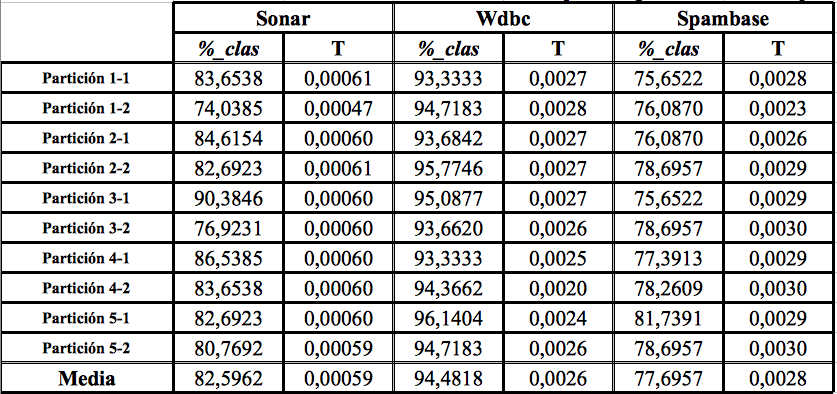
\includegraphics[scale=0.375]{1NN.png}  
	
}%

\noindent
\makebox[\textwidth]{
	\centering
	\label{fig: Resultados RELIEF}
	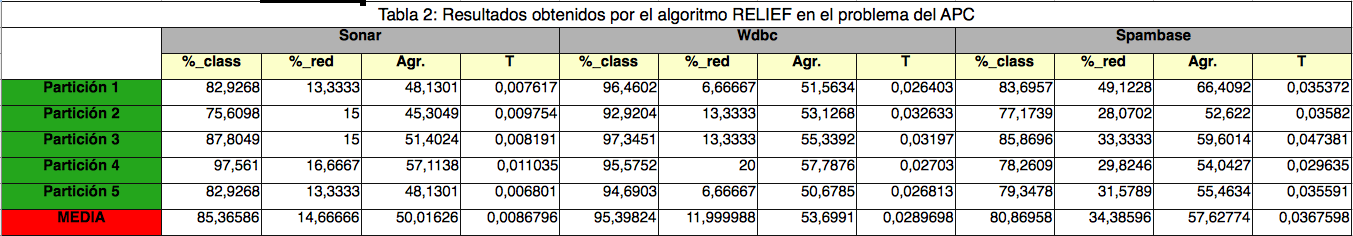
\includegraphics[scale=0.375]{RELIEF.png}
	
}%


\noindent
\makebox[\textwidth]{
	\centering
	\label{fig: Resultados SA}
	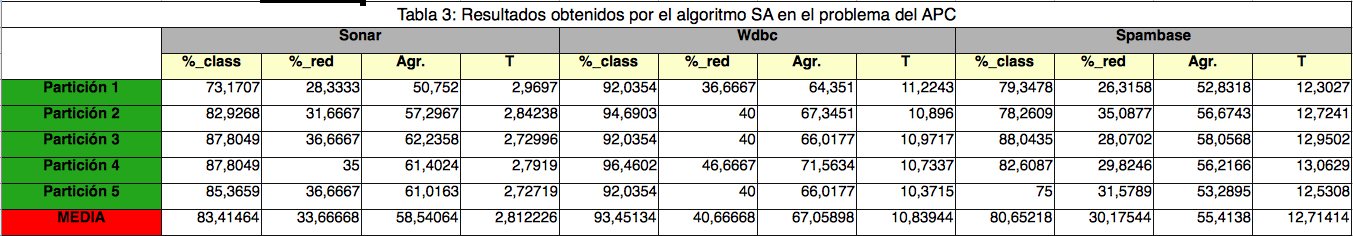
\includegraphics[scale=0.375]{SA.png}  
	
}%


\noindent
\makebox[\textwidth]{
	\centering
	\label{fig: Resultados ILS}
	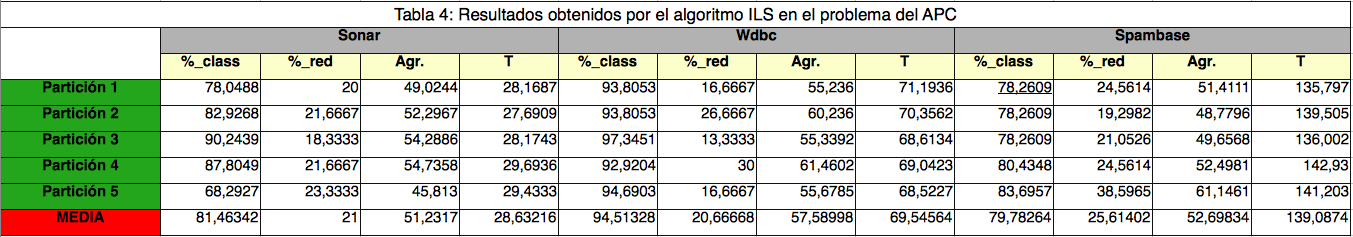
\includegraphics[scale=0.375]{ILS.png}   
	
}%


\noindent
\makebox[\textwidth]{
	\centering
	\label{fig: Resultados DE-RAND}
	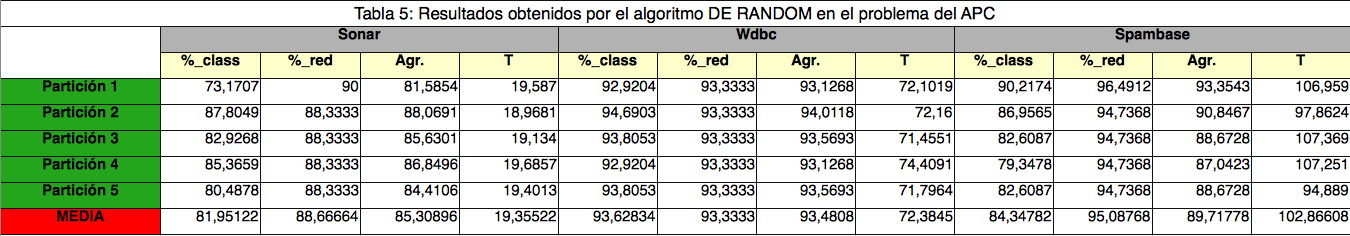
\includegraphics[scale=0.375]{DE-RAND.png}    
	
}%

\noindent
\makebox[\textwidth]{
	\centering
	\label{fig: Resultados DE-CURRENT-TO-BEST}
	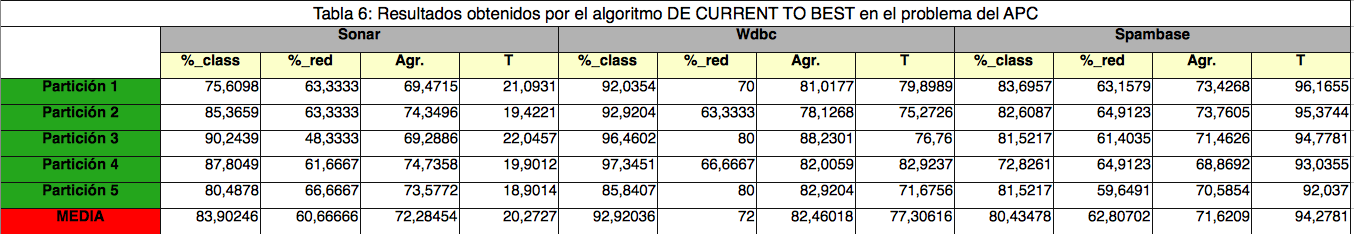
\includegraphics[scale=0.375]{DE-CURRENT-TO-BEST.png}     
	
}%

\noindent
\makebox[\textwidth]{
	\centering
	\label{fig: Resultados BL}
	\includegraphics[scale=0.375]{BL.png}  
	
}%

\noindent
\makebox[\textwidth]{
	\centering
	\label{fig: Resultados AGG-BLX}
	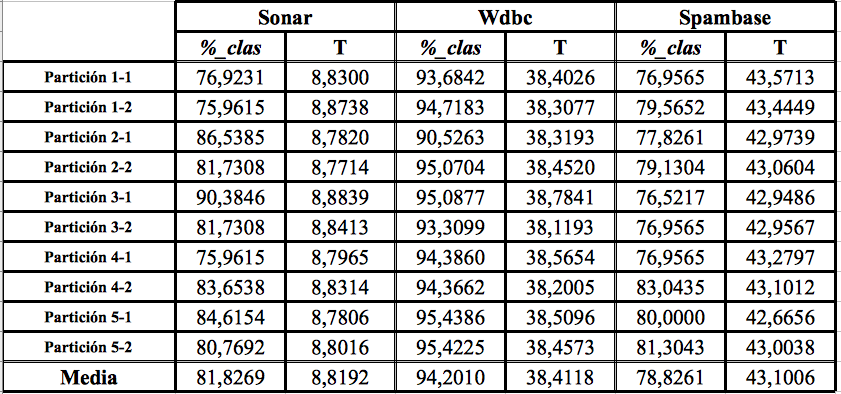
\includegraphics[scale=0.375]{AGG-BLX.png}   
	
}%



\noindent
\makebox[\textwidth]{
	\centering
	\label{fig: Resultados AM-01MEJ}
	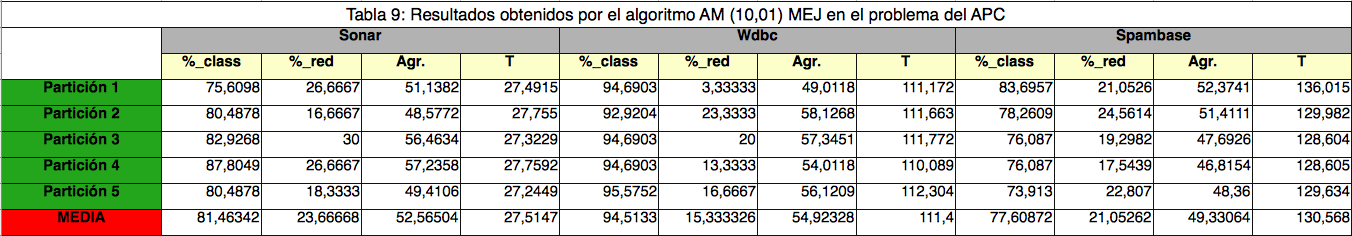
\includegraphics[scale=0.375]{AM-MEJ.png}       
	
}%






Ahora pasemos a realizar una tabla comparativa con las medias, tanto de tiempo como de tasas obtenidas para cada uno de los algoritmos para poder realizar así un análisis de forma global:

\noindent
\makebox[\textwidth]{
		\centering
		 \label{fig: Comparativa Global}
		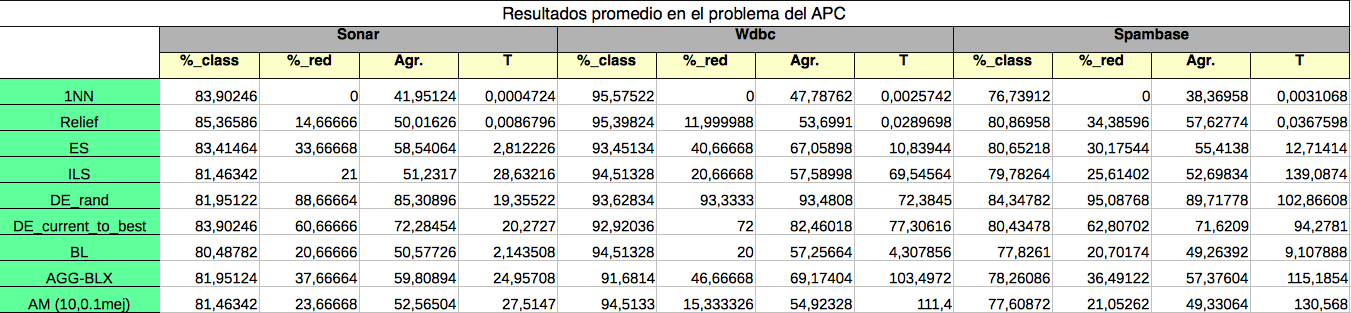
\includegraphics[scale=0.375]{PROMEDIO.png}  

}%


Realicemos ahora un análisis de los datos obtenidos e intentemos razonar el porqué de dichos datos.\\ 

Si analizamos a primera vista las tasas obtenidas según los tres distintos conjuntos, lo primero que nos damos cuenta es de la gran importancia que tiene el mero hecho de que el conjunto de datos que usamos sea o no representativo\\ 
Por ejemplo, nos damos cuenta de que el conjunto de datos de cáncer (Wdbc) es el que posee los datos más representativos de los tres, lo cuál facilita el aprendizaje. Es por eso que es en este en el que se obtienen las mayores tasas de clasificación, seguidas por las de Sonar y por último las de Spam. 


\subsection{Clasificación, Reducción y función objetivo}
Si observamos únicamente los valores obtenidos respecto a función objetivo, son los algoritmos de evolución diferencial los claros vencedores, elementalmente porque producen una alta tasa de reducción, lo cuál agrega a la función objetivo.

Si analizamos las tasas de reducción generadas por todos los algoritmos analizados, observamos que el claro vencedor es el algoritmo de evolución diferencial que emplea el esquema DE/Rand, superando casi en el doble al segundo mejor algoritmo. \\ 
Esto se debe básicamente a la aleatoriedad a la hora de la obtención del vector de mutación.
\\ 
Respecto a tasas de clasificación, como en la práctica anterior, los valores son muy similares, el vencedor en este caso el la evolución diferencial con modelo DE/current-to-best. 

\subsection{BL VS ILS}
Comparemos estos dos métodos de búsqueda. El segundo método consiste básicamente en aplicar una poca de exploración al algoritmo básico de BL, mediante el empleo de componentes aleatorias y mutaciones sobre la solución. Aunque el grado de exploración no es comparable al resto de algoritmos como DE o AGG, si analizamos la función objetivo tanto de BL como de ILS, observamos que de media tanto ILS como BL obtienen los mismos valores en tasas de clasificación, reducción y función objetivo. \\ 
Esto se debe en parte a lo descrito anteriormente, ambos tienen un máximo de 15000 llamadas a la función de evaluación.\\ 
La principal diferencia entre los dos es el proceso de diversificación que introduce la ILS, cosa del que BL carece, por eso en parte, las tasas son muy ligeramente superiores en ILS, en cambio el tiempo de ejecución se ve afectado en esta última.


\subsection{DE/rand VS DE/current-to-best}
Veamos ahora más detenidamente a los claros vencedores, los algoritmos de evolución diferencial.
Observando los resultados obtenidos, el claro vencedor es DE/rand. Pero si analizamos con detalle, esto es porque básicamente por que es capaz de obtener una tasa de reducción mucho superior a la obtenida por Rand; debido a la componente de aleatoriedad, sobre el esquema de cruce, lo cuál produce una mayor reducción a la hora de clasificar los datos.\\ 

Aunque los dos clasifican con un mismo error los datos, a la hora de elegir un modelo de aprendizaje, se antepone la simplicidad del modelo, es decir, dado dos soluciones iguales (o casi), aquella que sea la más simple siempre es la mejor. Por tanto, DE/Rand sería el modelo a escoger.\\ 

Aún así, si deseamos darle más importancia a la simplicidad, lo lógico sería que a la hora de calcular la agregación, aumentaremos el parámetro (porcentaje) de importancia a la tasa de reducción, en vez de dejarla en 0.5.


\subsection{Diversidad VS Convergencia}
Si comparamos evolutivos y enfriamiento simulado con la búsqueda local reiterada y la búsqueda local estrictamente observando la tabla, podríamos pensar que ambos son iguales en términos de tasa de clasificación, puesto que tanto los tiempos como las tasas obtenidas en los tres conjuntos no difieren apenas en unas décimas o incluso centésimas entre ellos.\\ 

Pero si analizamos la funcionalidad de ambos, podemos deducir que la principal diferencia entre los dos es la diversidad que producen. \\ 
En ILS así como BL, realizamos en el primero un proceso de diversificación modesto mediante mutación, mientras que en este último unicamente divergencia. \\ 

En cambio en los DE, se le da mayor énfasis a el cruce entre individuos de la población, y en ES a la reducción de la temperatura,  ampliando así el espacio de búsqueda. \\ 
En cualquier caso, una hibridación como la dada en el algoritmo memético es una buena opción para obtener un equilibrio entre diversidad y convergencia.



\section{Conclusión}
Como hemos visto en el análisis, la elección de un buen algoritmo de búsqueda es importantísima a la hora de la resolución de un problema, y se encuentra muy ligada a el ámbito de el mismo.\\ 

DE es un claro vencedor, debido principalmente al énfasis dado a la reducción de parámetros. 
Como anotación culmen, hemos de enfatizar la importancia de encontrar un equilibrio entre diversificación y convergencia.


%----------------------------------------------------------------------------------------
%	CODIGO EJEMPLO
%----------------------------------------------------------------------------------------

\begin{comment}


\begin{lstlisting}[language=bash, style=r]
warehouses=4
loadWorkers=4
terminals=1
//To run specified transactions per terminal- runMins must equal zero
runTxnsPerTerminal=0
//To run for specified minutes- runTxnsPerTerminal must equal zero
runMins=10
//Number of total transactions per minute
limitTxnsPerMin=300

//Set to true to run in 4.x compatible mode. Set to false to use the
//entire configured database evenly.
terminalWarehouseFixed=true
\end{lstlisting}

\end{comment}


%----------------------------------------------------------------------------------------
%	FIGURA
%----------------------------------------------------------------------------------------

\begin{comment}


\begin{figure}[H]
	\centering
	\includegraphics[scale=0.35]{cpu_utilization1.png}  
	\caption{Uso de la CPU, mejorado} 
\end{figure}


\end{comment}
%----------------------------------------------------------------------------------------
%	TABLA (ancho fijo)
%----------------------------------------------------------------------------------------

\begin{comment}

\begin{table}[htb]
\centering
\begin{tabular}{| p{2.2cm}| p{2.2cm} |  p{2.2cm} |}
\hline
\multicolumn{3}{|c|}{Europa} \\
\hline
\multicolumn{2}{|c|}{Localización} & Estado \\
\hline \hline
España & Madrid & Canada \\ \hline
España & Sevilla & EE.UU \\ \hline
Francia & París & Inglaterra \\ \hline
\end{tabular}
\caption{Tabla de ancho fijo.}
\label{tabla:Título de tabla}
\end{table}

\end{comment}


\bibliographystyle{plain} % hay varias formas de citar



\end{document}
